\documentclass[a4paper]{article}
\usepackage[utf8]{inputenc}
\usepackage{graphicx}

\usepackage[most]{tcolorbox}
\usepackage{lmodern}
\usepackage{lipsum}

\usepackage{tikz-qtree}
\usepackage{tikz}


\usepackage{subfiles} % Best loaded last in the preamble

% Keywords command
\providecommand{\keywords}[1]
{
    \small
    \textbf{\textit{Keywords: }} #1
}

% Document format: https://warwick.ac.uk/fac/sci/dcs/teaching/material/cs310/components/final/format/

\title{Butter: An efficient decentralised platform}
\author{Alexandre Shinebourne}
\date{December 2021}



\begin{document}

\maketitle

% Can I talk in the first person
% TODO: I need a clear definition of distributed vs decentralised system (taken from the Tanenbaum book)

\begin{abstract}
    Butter is a decentralized platform for building pure (unstructured) peer-to-peer systems.
\end{abstract}

\textbf{Keywords:} Networks, Decentralised, Unstructured peer-to-peer, Information retrieval, Persistent data

\tableofcontents

\section{Introduction}
% Use stuff from principle of distributed systems textbook - use it to make an overview of distributed systems section - re-iterate the summary from the introduction and architecture part

\section{Motivations}

\section{Background}
\begin{figure}
    \centering
    \subfile{distributedSystemsTaxonomy.tex}
    \caption{Distributed systems taxonomy}
    \label{fig:dis-taxonomy}
\end{figure}

This taxonomy clears up a lot of the confusion for me centralised systems e.g. a conventional web app with database, data processing backend and frontend is a distributed system but it is centralised as if the database becomes unavailable the app ceases to deliver any data. A centralised distributed system architecture is powerful because it decauples function into its logical components but create precarious systems with inherent interdependability.
Figure \ref{fig:dis-taxonomy} is not exaustive for example Distributed hash tables are not the sole means of designing overlay networks (wrappers around the network that allow the user to interface with it) but serves to give a general overview of distributed systems.


% Important terminology
% Overview of the history of distributed systems
% Overview of the academic field of distributed systems
% What are the problems to solve when building a distributed system?
% Different distributed architectures
% There are three big non-trivial problems that we are going to focus on:
% - Information retrieval in distributed systems (focus on IR in pure unstructured networks)
% - Information distribution in distributed systems (focus on pure unstructured networks)
% - Known host selection in distributed systems (focus on pure unstructured networks)
\subsection{Establishing a common language}\label{subsec:establishing-a-common-language}
The definition for distributed system is given to use by Tannenbaum and Van Steen in "Distributed systems Principles and Paradigms". They also make allusion to the general poor quality of definitions and lack of concensus so we use their loose characterization: "A distributed system is a collection of independent computers that appear to its user as a single coherent system."
There are two important aspects to this definition, first that a distributed systems consist of components that are autonomous and secondly that the user (person or program) view the system as a single coherent system (overlay network). The autonomous layer of the distributed system requires collaboration and establising that collaboration is the crux of designing any form of distributed system.

There are a few notable characteristics of distributed systems, given the defition
- "teh difference between the various computers and the way in which communicate are mostly hidden from the user"
- the user is not aware of the underlying architecture/organisation of the system
- "the user and application and applications can interact with a distributed system in a continous and uniform way, regardless of when and where the interactions take place
This is what makes distributed systems so powerful and such a good design for critical applications available over the internet - as a "distributed system should normally be contiously available" it should be detached from the underlying use/data it handles.

In order to support all manner of computers and networks while offering a single coherent interface for the system, distributed systems are typically organised into logical layers - with a high-level user and application layer, a low level operating system and basic commuinication layer - the distributed behaviour lies in-bitween hence is often reffered to as the distributed behaviour middleware.

\begin{figure}
    \centering
    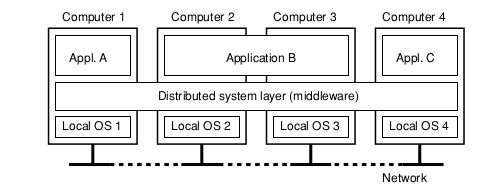
\includegraphics[width=0.8\textwidth]{imgs/Screenshot from 2022-01-17 17-13-57.png}
    \caption{Example of a distributed system with three logical layers}
    \label{fig:example-distributed-system-layers}
\end{figure}

The figure\ref{fig:example-distributed-system-layers}, taken from the Tanenbaum Steen book, shows four network connected computers, the distributed behaviour middleware (provided as a consistent interface between the operating systems and applications) and the top level application layer. Where application B is shared across computers 2 and 3.

stributed systen architectures - decentralised architecture: structured and unstructured peer-to-peer architectures



This whole section is taken from the Tanenbaum Steen book\cite{tanenbaumSteen}. % If your entire paragraph is paraphrase of info you got from one of your sources, just put the citation at the very end

This is an aggregation of all the common terminology that may be required when discussing decentralised systems.
\begin{itemize}
    \item A 'server' becomes a 'listener'
    \item A 'client' becomes a 'caller'
    \item A node is an entity on the network that can both call and listen (expressed as a vertec)
    \item A peer is a node connected to other nodes on the network (expressed as a vertex with at least one connection)
    \item Peers are two or more connected nodes
    \item Each peer has a list of known peers
    \item A first-degree peer is one that a peer has in his list (expreesed as as edge)
\end{itemize}

\section{Literature review/survey}
\section{Survey of current and past decentralised platform project}
% Survey of the decentralised platforms/project/products
%low level p2p libraries - developer centric libraries: libp2p, DAT project, maidsafe network...?
%high level products - user-centric: IPFS, FileCoin, Ethereum, Beaker browser..., BitTorrent

\section{Design}
% talk about the butter platform taxonomy
Problem centric design to buidding a sitributed system with as decentralised unstructured peer-to-peer architecyure
There are some problems specific to pure unstructure peer-to-peer architecture - where choosing known hosts, information retrieval and fault-tolerant persistent data storage become non-trivial problems.

\begin{figure}
    \centering
    \subfile{platformLayers.tex}
    \caption{Butter platform taxonomy}
    \label{fig:butter-platform-taxonomy}
\end{figure}

\begin{figure}
    \centering
    \subfile{platformLayersAbstracted.tex}
    \caption{Butter platform taxonomy abstracted}
    \label{fig:butter-platform-taxonomy-abstracted}
\end{figure}

Figure \ref{fig:butter-platform-taxonomy} neatly shows how teh platform lies in the wider network stack. The top layer is a user defined application and the developer interacts with a butter node - this abstracts away all teh underlying behaviour that handles the distributed aspects of the system. 

\subsection{Peer discovery}
\subsection{NAT traversal}
\subsection{Information retrieval in a pure unstructured network}
% Use the analogy of finding a book in a library with no apparent organisation scheme
% talk about being restricted to local knowledge and a partial view of the network (known hosts)
% even enforcing an alphabetical scheme to help make retrieval faster would require centralisation as we would need a node to allocate letters of the alphabet to each node entering the network
% There is a distinction between getting information when you known exactly what you are looking for (searching for something by a unique name/id) vs searching for something more generally i.e. search engine (both use search algorithms)
\subsection{Information distribution in a pure unstructured network}
\subsection{Known host selection in a pure unstructured network}

\section{Testing}

\section{Results}

\section{Evaluation}

\section{Project management methodology} % - like how the project was managed and carries out?
Poor choice of language to start with. At the beginning stages of the project the main focus should have been on designing the underlying algorithms for the purely unstructured peer-to-peer network. By starting in Rust, prototyping was slow and reasoning was more difficult as syntax an memory management got in the way of the design work. After switching to Go (which was done a little late in the projects life-cycle) the rate of progress increased massively.

\section{Future work}

\section{Legal, social and ethical discussion}
% How does the technology affect society?
On a personal note, I find a centralised internet a worrying place. There is a fragility to it and opportunities for abuse (maybe sometimes not conciously). This is why I feel so strongly about building on decentralised systems. Here individuals are protected not by rules or regulations (that may not always be enforced) but rather by the inherent design of the system. It is self-maintaining and open in its very nature. There is also a robustness to decentralised systems as we are avoiding single points of failure be it from a technology standpoint or a high level company/service standpoint
\section{Self-reflection}
\section{Acknowledgements}
\section{Conclusion}
\bibliographystyle{plain}
\bibliography{refs} % Entries are in the refs.bib file
\end{document}


% Unstructured peer to peer architecture
% searching in an unstruvtured overlay network

%Motivation
%This project was started as an effort to make a truly distributed system (or at least as close as possible) as "I" was
%not comfortable with the other offerings... I want to make a platform by design that reassures that data will be
%maintained and devoid of control. I want users to feel that they have no dependability. There has to be no universally
%known host within the data-layer (there are a few universally known host that are used simply during the startup
%procedure to allow NAT traversal.

%  Want to get as close as possible to a pure distributed system
%
%The resulting systems is an Unstructured p2p is arguably true p2p…
%
%Defined as having sorta random known peer list per node (we'll see that here this is not the case)
%
%The network also has to be efficient so not storing to many peers and not too much redundant data without risking data loss
%
%When dealing with persistent data on the network i.e. data blocks we need to be able to find them in a way that is totally decentralised - overlay network (nothing for it other than a more sophisticated bfs)

%// before I start the data layer of the p2p network TCP, I need to go through the start up
%// procedure to make at least one connection to the network

% Not only do I want to have a diverse set of known hosts (peers) in terms of uptime (hosts that I can rely on and hosts than can rely on me) but I also want to have a set of known hosts with a diverse set of knowledge/information to increase my probability of quickly finding information

% Choosing a language proved really defaut toyed with Rust, Go, Java, Javascript, Swift - but chose rust
% It is well suited high perfoance, low footprint

% Bceause Rust is hard the learning resources are really good - rust book, rust by example and realy active rust community

%The project's unique design approach is to think about events (meeting a new peer, interacting with a peer, conversing with a peer, spreading information) on the network in a social way, drawing inspiration from modelling human interaction in a social context. The information on the network should emulate the way humans naturally meet, communicate and dissipate information. A social gathering (e.g. a party or a casual meeting of friends) is arguably a good model of decentralised communication and hence can be drawn upon as inspiration.

% abstracting away most of the decentralised behaviour

% in the design section on information retrievel - maybe talk about the finding a book in a library analogy

% metatlity is everyrime you make a request infer as much data you can from it about the netwrok to reduce the need of surplus requests

%// block geo tag will be used to distribute replicated data geographically to reduce latency and avoid replicated data
%//sharing infrastructure (more robust)

% Explain what an overlay network is? Am I gona use an overlay network for information retrieval? No, I don't think so

% an important part of the design is that at all costs we do not want to stop a node - so even if operation fail e.g. a known host becomes innactive, we do not exit. Instead we handle all errors (think of a fail-operatoinal model). A node can only provide value if he is active - so we want to maximise uptime